\documentclass[../PianoDiQualifica.tex]{subfiles}
\begin{document}
	\section{Architettura generale}
		\progetto\ è realizzato utilizzando un'architettura client-server, in particolare:
		\begin{itemize}
			\item Il \textbf{client} corrisponde alla parte dell'applicativo che funzionerà nel
			browser dell'utente;
			\item Il \textbf{server} avrà il compito di fornire la pagina dell'applicativo al client
			e ne gestirà le richieste ricevute riguardanti la generazione del codice sorgente o le
			attività "bubble" da inserire nell'editor.
		\end{itemize}
		% INSERIRE IMMAGINE ARCHITETTURA CLIENT-SERVER GENERALE
		\subsection{Architettura client}
			Il client (parte \gl{front-end}) è una Single Page Application (\gl{SPA}) scritta con i linguaggi
			HTML5, \gl{CSS} e Javascript.\\
			La sua architettura è costruita utilizzando il framework Backbone.js che offre
			un'architettura di tipo Model-View ed è quindi principalmente suddivisa nei seguenti moduli:
			\begin{itemize}
				\item \textbf{Model}: organizza la logica alla base dei diagrammi dell'editor.
				\item \textbf{View}: gestisce l'interfaccia grafica dell'editor e, seguendo la struttura
				definita da Backbone.js, "contiene" la componente controller per la gestione
				degli eventi; 
			\end{itemize}
			% IMMAGINE ARCHITETTURA CLIENT GENERALE
			\begin{figure}[H]\label{fig:ClientSubsystem}
				\centering
				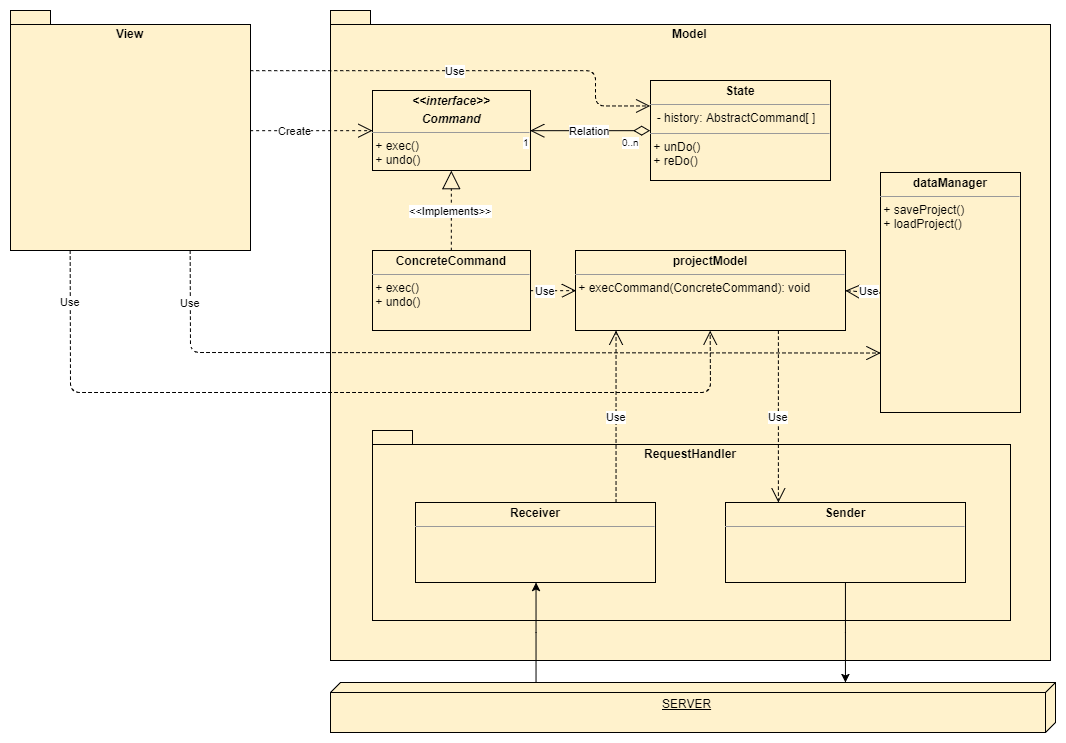
\includegraphics[scale=0.46]{Immagini/DiagrammaArchitettura/ClientSubsystem.png}
				\caption{Architettura del client}
			\end{figure}
			\subsubsection{Diagrammi editabili}
				In ogni diagramma creabile all'interno dell'applicazione è offerto solamente un
				sottoinsieme del totale dei formalismi definiti dal linguaggio UML standard.
				Si possono individuare tre tipi di diagrammi:
				\begin{itemize}
					\item Diagramma dei \gl{package};
					\item Diagramma delle classi;
					\item Diagramma delle bubble.
				\end{itemize}
				Il diagramma dei package è logicamente correlato con il diagramma delle classi. Per ogni
				elemento (package o classe) all'interno di questi diagrammi è possibile assegnare un
				livello di importanza attraverso il quale si può "filtrare" gli oggetti a schermo
				visualizzabili nell'editor.\\
				Per la corretta generazione del codice, nei diagrammi delle attività è previsto che
				l'utente approfondisca il loro livello di astrazione fino ad arrivare ad un diagramma
				costituito solamente da bubble (diagramma delle bubble) che verranno fornite nell'editor
				come se fossero delle attività specifiche.
		\subsection{Architettura server}
			Il server (parte \gl{back-end}) è sviluppato in Node.js ed offre i seguenti servizi:
			\begin{itemize}
				\item Fornire la Single Page Application ai client che la richiedono;
				\item Fornire la lista di bubble utilizzabili nell'editor;
				\item Generare il codice sorgente, nel formato desiderato dal client, del progetto
				inviatogli.
			\end{itemize}
			In particolare, la componente che genera il codice sorgente è stata realizzata utilizzando
			un'architettura di tipo Pipe And Filter, in modo tale da assegnare un compito ben preciso
			ad ogni modulo per attuare una procedura sequenziale a "catena di montaggio". L'ultimo
			modulo ha il compito di creare un file compresso .zip del codice generato che sarà poi
			inviato al client.\\
			Le bubble saranno salvate in una base dati per poter garantire una futura estendibilità del
			numero di queste ultime, eventualmente anche in altri domini da quello considerato al
			momento (i giochi da tavolo).
			% IMMAGINE ARCHITETTURA SERVER GENERALE
			\begin{figure}[H]\label{fig:ServerSubsystem}
				\centering
				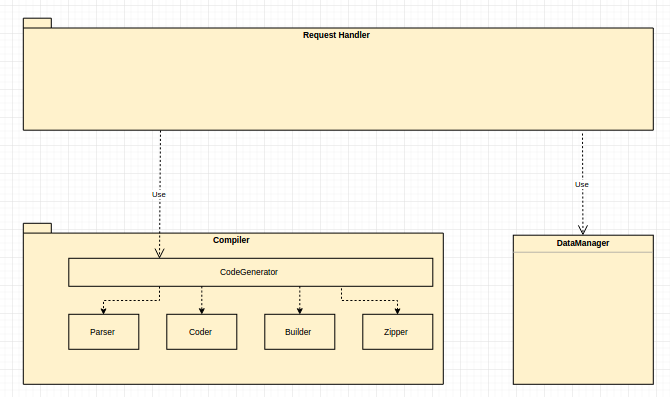
\includegraphics[scale=0.4]{Immagini/DiagrammaArchitettura/ServerSubsystem.png}
				\caption{Architettura del server}
			\end{figure}
			\subsubsection{Comunicazioni server-client}
				La Single Page Application viene fornita al client semplicemente attraverso una
				pagina HTML.\\
				Per la richiesta e fornitura delle bubble, client e server utilizzano AJAX per lo
				scambio di dati in formato JSON in modo tale da alleggerire il traffico.\\
				Per la richiesta della generazione del codice, il client invia i dati del progetto
				in formato JSON utilizzando AJAX ed il server una volta elaborata la richiesta procede
				con l'inviare il file .zip precedentemente descritto.
				\begin{figure}[H] \label{fig:ClientServerCommunications}
					\centering
					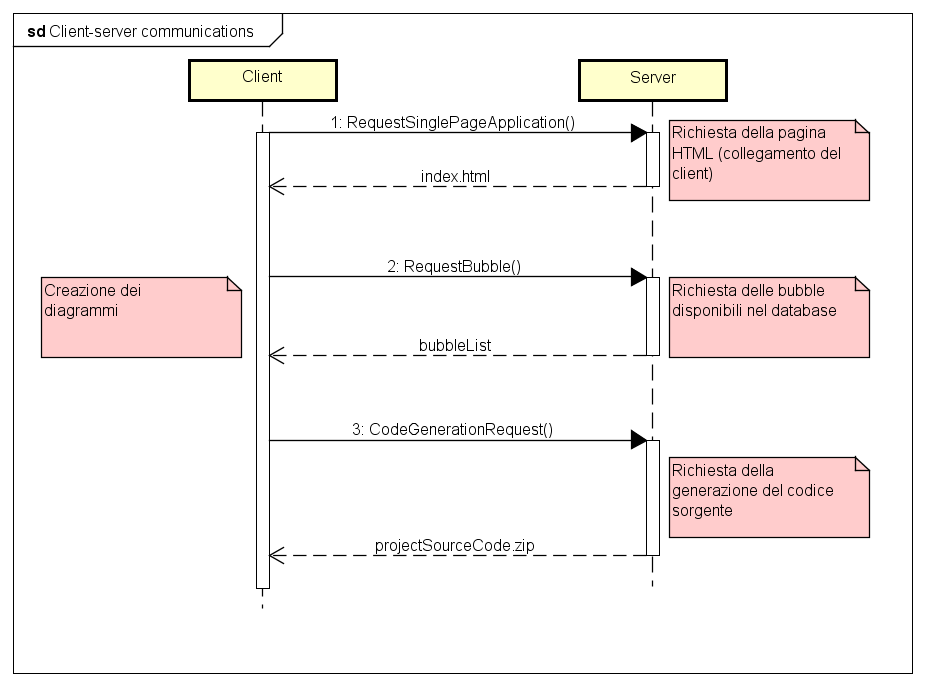
\includegraphics[scale=0.4]{Immagini/ClientServerCommunications.png}
					\caption{Esempi delle possibili comunicazioni client-server}
				\end{figure}
\end{document}